\documentclass{mcmthesis}
\mcmsetup{CTeX = false,   % 使用 CTeX 套装时,设置为 true
        tcn = 55869, problem = E,
        sheet = true, titleinsheet = true, keywordsinsheet = true,
        titlepage = false, abstract = true}
\problem{E}

\usepackage{palatino}
\usepackage{lipsum}
\usepackage{mwe}
\usepackage{graphicx}
\usepackage{tabularx}
\title{}
\date{}

\begin{document}

\begin{abstract}%摘要
In recent years, with the rapid development in economy and explosive growth in population, environment pollution and depletion of resources have been aggravated day by day. Smart Growth was then put forward. Lots of cities have drawn up the development plans on basis of the combination of ten principles for Smart Growth and their own conditions. Our work is to evaluate the success of each city in Smart Growth and provide a guidance for plan making.Meanwhile, we need to measure the success of our smart growth plan. Therefore, we define the "Smart Growth Index" (SGI) to measure the success of smart growth and development plans of a city. \\
\indent  Our model establishes a detailed group of 52 indictors, which reflects the ten principles for smart growth and the three E's of sustainability. On basis of this, we can assess the success of smart growth of a city. In the construction of SGI model, we use linear aggregation to combine individual variables into the theme scores. Compensability of linear aggregation ensures fair assessment of different cities which have different emphasis in urban development. Then we use geometric aggregation to combine theme scores into SGI. Low compensability of geometric aggregation requires a city to develop evenly in all themes. We use entropy method to determine weights of indictors or themes, which avoid subjectivity. SGI model has an all-round and objective assessment of the success of smart growth of a city.\\
\indent  With the completion of these, we respectively select a city in China and America (Zhenjiang and Columbia.SC). We assess the success of city development and their smart growth on basis of SGI model. 
Finally, we proved the reasonability and applicability of our model.\\
\begin{keywords}
 {\bf{Geometric and linear aggregation ;  entropy method} }\par
\indent\indent\indent\indent\indent {\bf Smart Growth Index ;  PCA}
\end{keywords}
\end{abstract}

\maketitle
\tableofcontents\thispagestyle{empty}
%设置页眉


\newpage
\setcounter{page}{1}
%Section 1
\section{Introduction}
\subsection{Background}%subsection 1.1
As is projected by 2050, 66 percent of the world's population will be urban, which means 2.5 billion people will be added to the urban population. Consequently, many communities are carrying out smart growth measures, which focus on the three E's of sustainability--Economically prosperous, socially Equitable, and Environmentally Sustainable, to ensure that people have access to equitable and sustainable homes, resources and jobs.
\subsection{Our work}
Smart growth is an urban planning theory that originated in 1990's as a means to curb continued urban expansion and reduce the loss of farmland surrounding urban centers.\\
To meet the requirements of ICM, we need to complete the following tasks:\\
{\bf (1) } Develop a metric model to measure the success of smart growth of a city based on the three E's of sustainability.\\
{\bf (2) } Use our model to measure and discuss whether the chosen two cities are successful in the current growth plans or meet the smart growth principles.\\
{\bf (3) } Develop a growth plan for both cities using smart growth principles, and explain why we chose these components and initiatives of plan from based on the geography, expected growth rates, and economic opportunities of the two cities. Assess whether our plans is successful or not by way of our model.\\
{\bf (4) } Use our models to rank the individual initiatives within our redesigned smart growth plan as the most potential to the least potential. Compare and contrast the initiatives and their ranking between the two cities.\\
{\bf (5) } Assess the applicability of our plans by supposing that the population of each city will increase by an additional 50\% by 2050.\\
\\
To further our solutions, we arrange our paper as follow:\\
In section 2, we make some reliable assumptions to simplify our metric model.\\
In section 3, we develop a model to measure the success of smart growth of a city.\\
In section 4, we develop a plan analysis model to assess smart growth plan. And, develop a metric to assess the importance of each initiative in a plan.\\
In section 5, solutions for tasks.\\
In section 6, sensitivity analysis.\\
In section 7, strengths and weaknesses\\

%Section 2
\section{Assumptions}
{\bf (1) } The real change of indictors corresponds to policies.\\
{\bf (2) } Each indictor will not have abrupt and rapid changes.\\
{\bf (3) } The relationship between initiative and indictor is one to one.\\
{\bf (4) } Indictors are mutually dependent.\\

%Section 3
\section{The Smart Growth Index Metric Model}
\subsection{Theoretical framework}%subsection 3.1理论框架
\subsubsection{framework}%3.1.1
\centerline{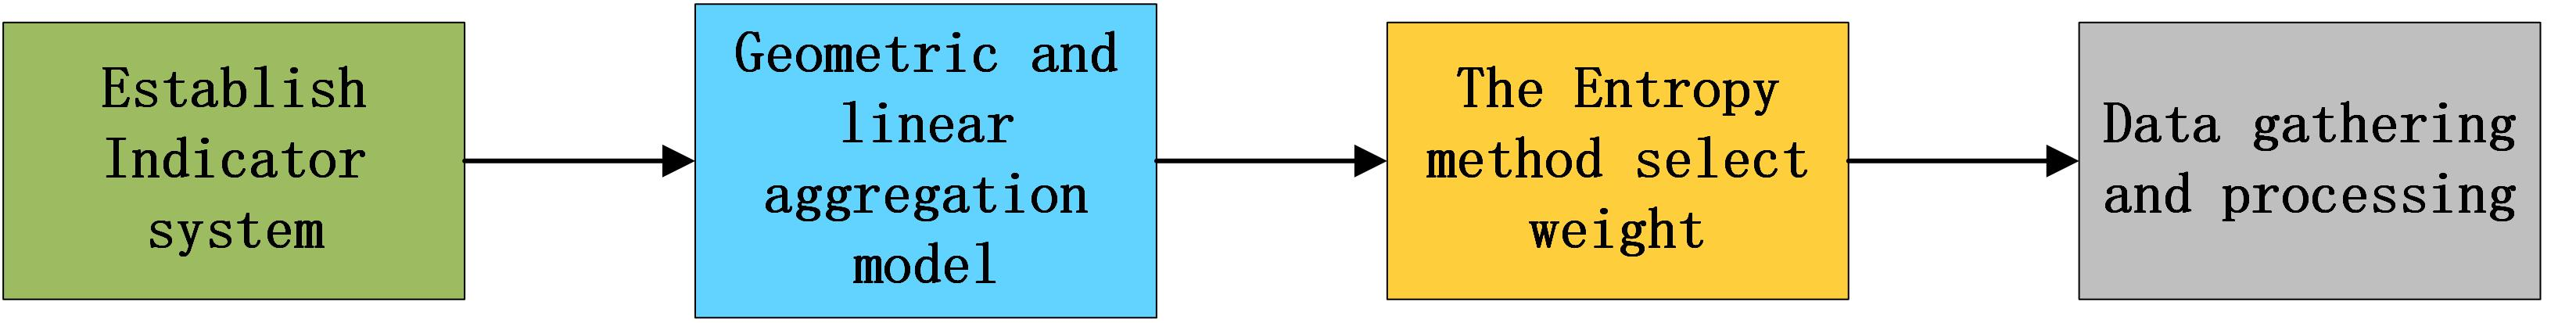
\includegraphics[height=1.8cm]{flow.jpg}}
\centerline{Figure1:Flow diagram}
To meet ICM group's requirements, we establish a model to access the smart growth of a city. Thus, we define an index as the criterion to measure the success of smart growth of a city, represented as SGI (Smart Growth Index).\\
Referring to literature  and research $^{[1]}$, we choose 52 indictors (including positive indictors and negative indictors), which have effects on SGI in degrees, based on the ten principles for smart growth and the three E's of sustainability. Through analysis, we further boil these indictors down to 4 themes. Finally, we aggregate the 4 themes as the SGI.\\
\newpage
\noindent Briefly, we can develop a three-layer model (outer: indictors; middle: themes; inner: SGI) based on the analysis above. Below are the figure reflecting the relationships:\\
\centerline{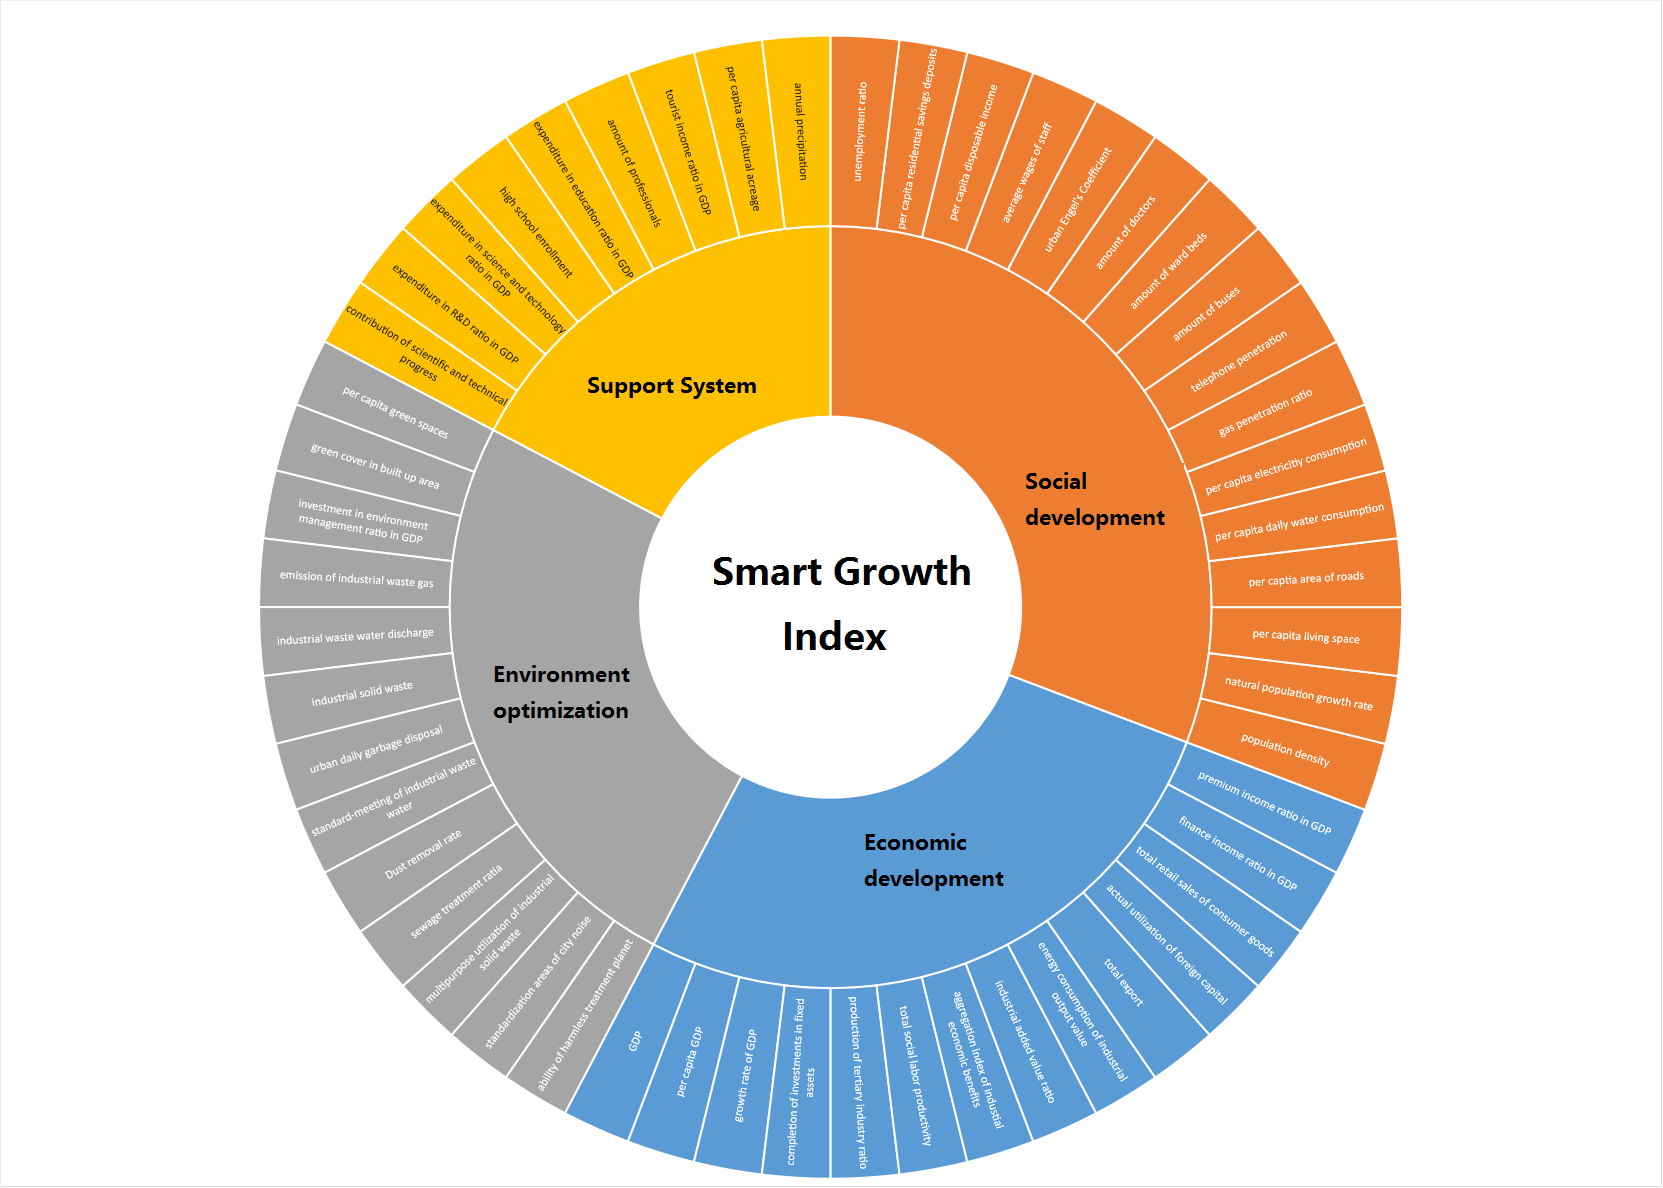
\includegraphics[height=15cm]{SGI.png}}
\centerline{Figure2:The relationship of the model }
\subsubsection{Multivariate Analysis by PCA}%3.1.2
After selecting indicators,we try to assess between-variable correlation by Principle Compomnents Analysis(PCA).\\
the results of the PCA fitted less closely with our conceptual framework for the Environment theme.
However ,because we think it's indicators we selecteed are importent , we left them unchanged.
\subsection{Construction of SGI Model}%subsection 3.2
\subsubsection{Geometric and linear aggregation model}%sub subsection 3.2.1线性几何
We decide to use GLA to obtain the relationship between SGI and the 4 themes along with 52 indictors.\\
Geometric and linear aggregations (GLA) each have their own benefits, while in a linear aggregation, the compensability is constant, with geometric aggregations, compensability is lower for the composite indictor or themes with low values. This means that when using a geometric aggregation, a city with a low score for one indictor or theme will need a much higher score on the others to improve its score.\\
Thus, it's relatively reasonable to use GLA to obtain the SGI. From indictors to themes, we use liner aggregation model. And, from themes to SGI, we use geometric aggregation model.\\
This captures the non-compensability across themes without making the Index too sensitive to individual variables for which the importance, robustness and compensability is less clear.The figure as follow:\\
\centerline{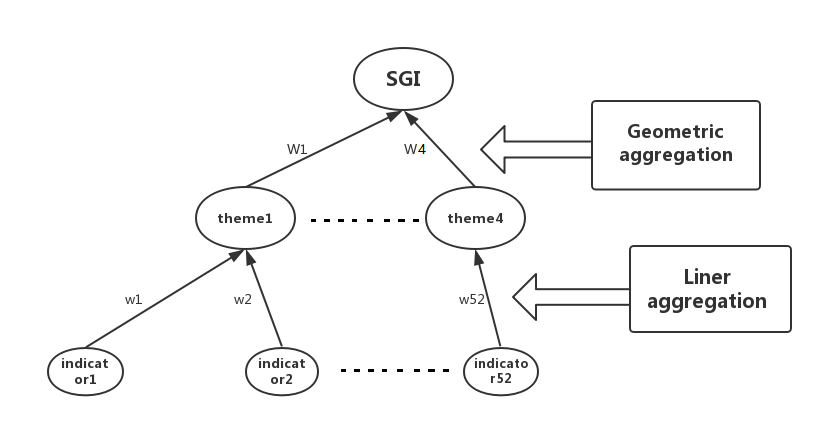
\includegraphics[height=9cm]{model.png}}
\centerline{Figure3:GLA model}
{\bf (1) } Liner aggregation equation for the score of theme\\
$$\bf T_{i}=\frac{\sum_{j=1}^{J}w_jz_{j}}{\sum_{j=1}^{J}w_j}$$
where $\bf T_{i}$is the aggrregated theme score for  theme i of chosen city\\
$\bf w_j$ is the weight given to indicator\\
$\bf z_{j}$ is the normalised value for  indicator j\\
{\bf (2) } Geometric aggregation equation for the score of SGI\\
$$\bf SGI=(\prod_{i=1}^{I}{T_{i}}^{W_i})^{\frac{1}{\sum_{i=1}^IW_i}}$$
where $\bf SGI$ is the aggregated Index score for the chosen city .\\
$\bf W_i$ is the weight given to theme .\\
$\bf T_{i}$ is the aggregated theme score for the theme.\\
In consideration of the different measurement of these indictors, we decide to normalize the data of indictors to a certain extent, in order to apply to the basic model above.\\
\subsubsection{Normalization}%sub subsection 3.2.2
Due to indictors measured in different counting units, we adopt a min-max normalization method which normalizes the 52 indicators within an identical [0,1] range.\\
Normalization equations\\
For positive indictors\\
$${z}_{j}=\frac{x_{j}-min (x_j) }{max(x_j)-min(x_j)}$$
For negative indictors\\
$${z}_{j}=\frac{max (x_j) -x_{j}}{max(x_j)-min(x_j)}$$
$\bf x_j$ represents the data of indictor j.\\
$\bf z_j$ represents  the data of indictor j after normalization.\\
\subsubsection{Weigh indictors and themes by Entropy method}%sub subsection 3.2.3
We adopt the Entropy method to determine the weight of each indictor or theme.\\
Entropy is originally a physical theory in thermodynamics. In information system, entropy weight, known as information entropy, reflects the disorder of information. The smaller  the information entropy is, the lower the disorder of information is, which means the availing value of information is great. And, the problem of weight allocation is solved. \\
Compared with other methods like AHP and so on, this way is more objective and more reliable to reflect the relationship between indictors or themes in the model. Below are the steps to determine the weight:\\
{\bf Step 1:} Choose n cities and m indictors. And $x_{ij}$ represents the data of indictor j of city i (i=1,2,3...n, j=1,2,3...m).\\
{\bf Step 2:}  Normalize indictors using the method in 3.2.2.$\bf z_j$ represents  the data of indictor j after normalization\\
{\bf Step 3:} Calculate the proportion $\bf p_{ij}$ of $\bf z_{ij}$
$$p_{ij}=\frac{z_{ij}}{\sum_{i=1}^nz_{ij}},i=1,...,n,j=1,...,m$$
{\bf Step 4:} Calculate the entropy $\bf e_j$ of variable j\\
$$e_j=-k\sum_{i=1}^np_{ij}ln(p_{ij})$$
$k=1/ln(n)>0,e_j\ge0$\\
{\bf Step 5:} Calculate the availing value $\bf d_j$ of variable j\\
$$d_j=1-e_j$$
{\bf Step 6:} Calculate the weight $\bf w_j$ of variable j\\
$$w_j=\frac{d_j}{\sum_{j=1}^{m}d_j}$$
{\bf Step 7:} Calculate the weight $\bf W_k$\\
According to Entropy's additivity, we can obtain the weight of theme(middle) on the basis of the availing value of variable(bottom). \\
Summarize the availing value of indictors, which correspond to theme k, and we obtain the availing value of theme k denoted by $D_k(k=1,2,3,4)$.then we obtain \\
$$D=\sum_{k=1}^4D_k$$
therefore\\
$$W_k=\frac{D_k}{D}$$
Based on the data of several cities over 10 years$^{[2]}$ ,we obtain the weight of each variable by the way of the entropy method\\


\begin{table}
\setlength{\abovecaptionskip}{0pt}
\setlength{\belowcaptionskip}{0pt}
\centering
\centering{Table 1:City Smart Growth indicator system weight}
\begin{tabular}{p{0.4cm}|p{9cm}|p{1.5cm}|p{1.5cm}|p{1.7cm}}
\hline
\bf I	& {\bf Indictors}			 &  \bf entropy		& \bf availing value		& \bf weight (\%) \\	
\hline
\rowcolor[gray]{0.9}	& Group of indictors for ecnomic development			& 		& 		& 22.925 \\	
\hline
 1		& GDP( 100 million yuan)		& 0.99001		& 0.00999		& 7.59925 \\	
2		& per capita GDP(yuan/person)		& 0.99044		& 0.00956		& 7.27817 \\	
3		& growth rate of GDP(\%)		& 0.99723		& 0.00277		& 2.11033 \\	
4		& completion of investments in fixed assets(\%)		& 0.99512		& 0.00488		& 3.71549 \\	
5		& production of tertiary industry ratio(\%)		& 0.99908		& 0.00092		& 0.70123 \\	
6		& total social labor productivity(yuan)		& 0.98483		& 0.01517		& 11.5444 \\	
7		& aggregation index of industial economic benefits		& 0.99766		& 0.00234		& 1.7815 \\	
8		& industrial added value ratio(\%)		& 0.99892		& 0.00108		& 0.8213 \\	
9		&energy consumption of industrial output value (tce)		& 0.99687		& 0.00313		& 2.37957 \\	
10		& total export(100 million dollars)		& 0.98463		& 0.01537		& 11.6974 \\	
11		& actual utilization of foreign capital(100 million dollars)		& 0.97431		& 0.02569		& 19.5481 \\	
12		& total retail sales of consumer goods(yuan)		& 0.99087		& 0.00913		& 6.9475 \\	
13		& finance income ratio in GDP(\%)		& 0.98757		& 0.01243		& 9.46227 \\	
14		& premium income ratio in GDP(\%)		& 0.98106		& 0.01894		& 14.4136 \\	
	&\bf  SUM			& 		& 0.1314		& 100 \\	
\hline
\rowcolor[gray]{0.9}	& Group of indictors for social development			& 		& 		& 32.8844 \\	
\hline
15		& population density(person/${km}^2$)		& 0.99998		& 0.000021		& 0.01095 \\	
16		& natural population growth rate(\%)		& 0.98577		& 0.01432		& 7.54951 \\	
17		& per capita living space(urban,$m^2$)		& 0.99927		& 0.00073		& 0.38819 \\	
18		& per captia area of roads(urban,$m^2$)		& 0.99469		& 0.00531		& 2.81685 \\	
19		& per capita daily water consumption(urban,L)		& 0.99739		& 0.00261		& 1.38275 \\	
20		& per capita electricitiy consumption(W)		& 0.983176		& 0.016824		& 8.926287 \\	
21		& gas penetration ratio(urban,\%)		& 0.99829		& 0.00171		& 0.90891 \\	
22		& telephone penetration(set/hundred person)		& 0.941254		& 0.058746		& 31.16803 \\	
23		& amount of buses (per ten thousand)		& 0.981269		& 0.01873		& 9.938145 \\	
24		& amount of ward beds(per ten thousand)		& 0.99656		& 0.00344		& 1.82491 \\	
25		& amount of doctors (per ten thousand)		& 0.99507		& 0.00493		& 2.61773 \\	
26		& urban Engel's Coefficient(\%)		& 0.99754		& 0.00246		& 1.30663 \\	
27		& average wages of staff(yuan)		& 0.98371		& 0.01629		& 8.64347 \\	
28		& per capita disposable income(urban, yuan)		& 0.99453		& 0.00547		& 2.89988 \\	
29		& per capita residential savings deposits(urban,yuan)		& 0.972096		& 0.027904		& 14.8049 \\	
30		& unemployment ratio(urabn,\%)		& 0.990929		& 0.009071		& 4.812845 \\	
	& \bf SUM			& 		& 0.188481		& 100 \\	
\hline
\hline
\end{tabular}
\end{table}

\begin{table}
\setlength{\abovecaptionskip}{0pt}
\setlength{\belowcaptionskip}{0pt}
\centering
\begin{tabular}{p{0.4cm}|p{8cm}|p{1.5cm}|p{1.5cm}|p{1.7cm}}
\hline
\bf I	& \bf Indictors			 &  \bf entropy		& \bf availing value		& \bf weight (\%) \\	
\hline
\rowcolor[gray]{0.9}	& Group of indictiors for environment optimization			& 		& 		& 22.6476 \\	
\hline
31		& per capita green spaces($m^2$)		& 0.9962		& 0.0038		& 2.927595 \\	
32		& green cover in built up area(\%)		& 0.994739		& 0.005261		& 4.052684 \\	
33		& investment in environment management ratio in GDP		& 0.946798		& 0.053202		& 40.98544 \\	
34		&  emission of industrial waste gas(billion cubic meters)		& 0.997865		& 0.002135		& 1.645014 \\	
35		& industrial waste water discharge(ten thousand ton)		& 0.99866		& 0.00134		& 1.032296 \\	
36		& industrial solid waste(ten thousand ton)		& 0.997948		& 0.002052		& 1.580738 \\	
37		& urban daily garbage disposal(ten thousand ton)		& 0.996143		& 0.003857		& 2.971568 \\	
38		& standard-meeting of industrial waste water(\%)		& 0.980095		& 0.019905		& 15.33443 \\	
39		& Dust removal rate(\%)		& 0.997501		& 0.002499		& 1.924922 \\	
40		& sewage treatment ratia(\%)		& 0.99454		& 0.00546		& 4.205913 \\	
41		& multipurpose utilization of industrial solid waste(\%)		& 0.995567		& 0.004433		& 3.414808 \\	
42		& standardization areas of city noise(${km}^2$)		& 0.983896		& 0.016104		& 12.40645 \\	
43		& ability of harmless treatment planet(ton)		& 0.990241		& 0.009759		& 7.518134 \\	
	&\bf  SUM			& 		& 0.129807		& 100 \\	
\hline
\rowcolor[gray]{0.9}	& Group of indictors for support  system			& 		& 		& 21543 \\	
\hline
44		& annual precipitation(mm)		& 0.991201		& 0.008799		& 7.126399 \\	
45		& per capita agricultural acreage(acre)		& 0.999253		& 0.000747		& 0.604674 \\	
46		& tourist income ratio in GDP(\%)		& 0.962193		& 0.037807		& 30.61872 \\	
47		& amount of professionals(ten thousand, person)		& 0.995093		& 0.004907		& 3.974089 \\	
48		& expenditure in education ratio in GDP		& 0.995912		& 0.004088		& 3.31051 \\	
49		& high school enrollment(ten thousand,person)		& 0.973031		& 0.026969		& 21.84158 \\	
50		& expenditure in three charges of science and technology ratio in GDP(\%)		& 0.985541		& 0.014459		& 11.70999 \\	
51		& expenditure in R\&D ratio in GDP(\%)		& 0.975452		& 0.024548		& 19.88107 \\	
52		& contribution of scientific and technical progress(\%)		& 0.998848		& 0.001152		& 0.932972 \\	
	&\bf  SUM			& 		& 0.123476		& 100 \\	
\hline
\hline
\end{tabular}
\end{table}



\newpage

%Section 4
\section{Analysis of chosen cities' smart growth}
\subsection{Construction of plan analysis model(PAM)}%subsection 4.1
We develop a metric model to assess the effects of a plan or policy on the SGI. Also, we can analysis the potential of indictors in a plan(policy) by the way of the model. \\
\subsubsection{Assumptions  for PAM}%sub subsection 4.1.1
{\bf (1) } Due to the established detailed group of indictors, we assume that the relationship between plan(policy) and indictor is one to one, even though the existence of the situation of n to one, we can also simplify the relationship as one to one on the basis of SGI model.\\
{\bf (2) } We assume that the relationship between plan(policy) and indictor is linear to simplify our model.\\
{\bf (3) }Quantification of plan(policy) is directly reflected in the data of indictors of a city.
The relationship between plan(policy) and indictor is reflected in data of years in a city.\\
\subsubsection{Plan's impacts  on SGI}%sub subsection 4.1.2
According to the researches on urban planning of a city, we know of its plans(policies), we can boil plans(policies) down to indictors or themes on the basis of assumptions above and linear aggregation model. \\
Thus, we can further analyze these plans'(or policies') impacts on SGI by the way of geometric aggregation model.\\
Below are the method\\
{\bf (1) } According to the plans or policies, we update data of relative indictors.\\
{\bf (2) } Using SGI model on the basis of new data of indictors, we can obtain a new smart growth index, represented as SGI'.\\
{\bf (3) } We can further obtain the change in SGI based on the original SGI of city(plans or policies not carried out). \\
$$\Delta SGI=SGI'-SGI$$
{\bf (4) } Through the analysis of ${\Delta SGI}_i$ , we can see the impacts of plans or policies on SGI.
\subsection{Assess the importance of initiatives in a plan}%subsection 4.2
A plan has many initiatives, which has different emphasis on various fields. Thus, we develop a metric to assess the importance of each initiatives. Below is the metric:\\
{\bf (1) } On the basis of APM, we can obtain SGI' after a plan is implemented.\\
{\bf (2) }  Then we adopt qualitative analysis, only implement an initiative of a plan($\bf e.g.$ initiative i), therefore, we can obtain a new index ${SGI_i}'$.\\
{\bf (3) } We can get the change in SGI\\
$$\Delta {SGI_i}'={SGI'}-{SGI_i}'$$
Through the qualitative analysis of each initiative, we obtain the change in SGI of each initiative.\\
{\bf (4) } Compare the relative change$|\frac{\Delta SGI'}{SGI'}|$ on the basis of original SGI', and we can analyze the importance of each initiative. \\

\newpage

%Section 5
\section{Solutions for tasks }
\subsection{Task 1}%subsection 5.1
We have developed our models in the section 3(SGI model) and section 4(PAM).\\
\subsection{Task 2}%subsection 5.2
According to the current researches on urban planning of our chosen cities (Columbia.SC and Zhenjiang), we adopt quantization analysis of plans or policies. Then we obtain the following policy conclusion:\\
%%政府政策
\begin{table}[h]

\centering
\centering{Table 2:Current Plan}
\begin{tabular}{p{5.2cm}|p{1.2cm}|p{5.2cm}|p{1.2cm}}
\hline
\bf Zhenjiang 5 years	 & \bf change	 & \bf Columbia 5 years	& \bf change \\
\hline
 per capita GDP(yuan/person)	& +8\%	& per capita disposable income( yuan)	& +5\% \\
production of tertiary industry ratio(\%)	& to 50\%	& per capita green spaces($m^2$)	& +4\% \\
per capita disposable income(yuan)	& +8.5\%	& average wages of staff(yuan)	& +5\% \\
tourist income ratio in GDP(\%)	& +100\%	& sewage treatment ratia(\%)	& to 99\% \\
total export(100 million dollars)	& +50\%	& high school enrollment(10000 person)	& +8\% \\
amount of doctors (per ten thousand)	& +10\%	& per capita living space($m^2$)	& +7\% \\
per captia area of roads(urban,$m^2$)	& +10\%	& green cover in built up area(\%)	& +5\% \\
\hline
\end{tabular}
\end{table}

\noindent Using SGI model, we can obtain SGI of two cities after implementing the current plan. Also, we can obtain original SGI on the basis of original data. Based on the method in section 4, we can get the following result by way of matlab.\\

%%政府政策中SGI总和
\begin{table}[h]
\setlength{\abovecaptionskip}{0pt}
\setlength{\belowcaptionskip}{0pt}
\centering{Table 3:SGI of Current Plan}
\begin{tabular}{p{3.3cm}|p{3cm}|p{3cm}|p{3.3cm}}
\hline
City	& $SGI_0$ (2014)	& $SGI$ (2020)	& $\Delta SGI$ \\
\hline
Zhenjiang	& 12.5126	& 14.3771	& 1.8645 \\
columbia	& 13.962	& 14.1089	& 0.1469 \\
\hline
\end{tabular}
\end{table}
%%
\noindent Through the analysis of the relative change in SGI of two cities, we can assess the success of the growth plan.\\
Apparently, SGI of two cities both increases after implementing their own current growth plan. \\
Thus, their current growth plan is both successful.\\
\subsection{Task 3}%subsection 5.3
\subsubsection{Our growth plans}%sub subsection 5.3.1
Combining the current plans of two cities and ten principles of smart growth, we make the following growth plans for our cities over few decades.\\
%%我们的计划
\begin{table}[h]
\setlength{\abovecaptionskip}{0pt}
\setlength{\belowcaptionskip}{0pt}
\centering{Table 4:Our Plan}
\begin{tabular}{p{5.3cm}|p{1.2cm}|p{5.2cm}|p{1.2cm}}
\hline
\bf Zhenjiang 10 years	& \bf change	 & \bf Columbia 10 years	& \bf change \\
\hline
 per capita GDP(yuan/person)	& +100\%	& per captia area of roads(urban,$m^2$)	& +15\% \\
production of tertiary industry ratio(\%)	& to 55\%	& ability of harmless treatment planet(ton)	& +100\% \\
total export(100 million dollars)	& +100\%	& tourist income ratio in GDP(\%)	& +100\% \\
per capita disposable income(yuan)	& +100\%	& amount of professionals(10000 person)	& +50\% \\
 per capita green spaces($m^2$)	& +20\%	& expenditure in education ratio in GDP	& to 10\% \\
 high school enrollment(10000 person)	& +100\%	& high school enrollment(10000 person)	& +50\% \\
total social labor productivity(yuan)	& +200\%	& amount of ward beds(per ten thousand)	& +30\% \\
amount of ward beds(per ten thousand)	& +20\%	& per capita green spaces($m^2$)	& +10\% \\
\hline
\end{tabular}
\end{table}

%%
\subsubsection{Reasons for choosing these initiatives}%sub subsection 5.3.2
Ten principles of smart growth can be reflected in the detailed of indictors. Thus, in the process of making our smart growth plans, we just need to choose appropriate indictors supported by policies on basis of geography and economic development.\\

\noindent For Zhenjiang, as manufacturing industry basement in middle and lower reaches of Yangtze River in China, adept in manufacturing and export, we can stimulate its export in our plan, which can accelerate the development of city. Even though economic development is on the agenda, the environment and medical level is as important as economic development. Thus, we also give priority to relative indictors of these elements in our smart growth plan. \\
For Columbia.SC, its economy and livelihood have higher level, thus we put its emphasis on education, technology and protection of environment. In the meanwhile, tertiary industry should be developed rapidly, which plays important role in urban development. \\
\noindent Therefore, we make these smart growth plans above for both cities. \\
\subsubsection{Assessment of the success of our smart growth plans}%sub subsection 5.3.3
Based on the method in task 2, we can obtain the changes in SGI of two cities by way of matlab after implementing our growth plans.\\
%%我们的计划中SGI总和
\begin{table}[h]
\setlength{\abovecaptionskip}{0pt}
\setlength{\belowcaptionskip}{0pt}
\centering{Table 5:SGI of Our Plan}
\begin{tabular}{p{3cm}|p{3cm}|p{3cm}|p{3cm}}
\hline
City	& $SGI_0$ (2014)	& $SGI$ (2025)	& $\Delta SGI$ \\
\hline
Zhenjiang	& 12.5126	& 15.4329	& 2.9023 \\
columbia	& 13.962	& 15.092	& 1.13\\
\hline
\end{tabular}
\end{table}

%%
\noindent Apparently, SGI of two cities both increases after implementing our smart growth plan. Therefore, our smart growth plans are successful in the chosen cities through analysis.\\
\newpage
\subsection{Task 4}%subsection 5.4
\subsubsection{Assessment of the importance of each initiative}%sub subsection 5.4.1
In this task, we need to rank our chosen initiatives of our smart growth plan. Thus, we can compare the importance of each initiative to complete this task.\\
On basis of the method mentioned in 4.2 of section 4 and SGI model, we can obtain the   following ranking of each city by way of matlab.\\
%%计划排名
\begin{table}[h]
\setlength{\abovecaptionskip}{0pt}
\setlength{\belowcaptionskip}{0pt}
\centering{Table 6:Ranking of initiatives}
\begin{tabular}{p{1cm}|p{7cm}|p{1.3cm}|p{1.4cm}|p{1.4cm}}
\hline
\hline
\rowcolor[gray]{0.9}\multicolumn{5}{c}{Columbia}\\
\hline
\bf rank & \multicolumn{2}{|c|}{ \bf  initiatives} & \bf SGI	&  \bf $\Delta SGI$ \\
\hline
1	& tourist income ratio in GDP(\%)	& +100\%	& 14.3194	& 0.3574 \\
2	& high school enrollment(10000 person)	& +50\%	& 14.2334	& 0.2714 \\
3	& ability of harmless treatment planet(ton)	& +100\%	& 14.1711	& 0.2090 \\
4	& amount of professionals(10000 person)	& +50\%	& 14.0586	& 0.0966 \\
5	& expenditure in education ratio in GDP	& to 10\%	& 13.9929	& 0.0309 \\
6	&  amount of ward beds(per ten thousand)	& +30\%	& 13.9838	& 0.0218 \\
7	& per capita green spaces($m^2$)	& +10\%	& 13.9811	& 0.0190 \\
8	& per captia area of roads(urban,$m^2$)	& +15\%	& 13.9726	& 0.0106 \\
\hline
\hline
\rowcolor[gray]{0.9}\multicolumn{5}{c}{Zhenjiang}\\
\hline
\bf rank & \multicolumn{2}{|c|}{ \bf  initiatives} & \bf SGI	&  \bf $\Delta SGI$ \\
\hline
1	& total export(100 million dollars)	& +100\%	& 14.4935	& 1.9809 \\
2	&  high school enrollment(10000 person)	& +100\%	& 13.0236	& 0.5109 \\
3	& per capita disposable income(yuan)	& +100\%	& 12.6755	& 0.1628 \\
4	& total social labor productivity(yuan)	& +200\%	& 12.6102	& 0.0975 \\
5	&  per capita GDP(yuan/person)	& +100\%	& 12.5504	& 0.0377 \\
6	& amount of ward beds(per ten thousand)	& +20\%	& 12.5304	& 0.0177 \\
7	&  per capita green spaces($m^2$)	& +20\%	& 12.5288	& 0.0161 \\
8	& production of tertiary industry ratio(\%)	& to 55\%	& 12.5128	& 0.0002 \\
\hline
\end{tabular}
\end{table}

%%
\subsubsection{Analysis of the ranking}%sub subsection 5.4.2
Evidently, the ranking proves the reasonability of our plans' emphasis.\\
The ranking of the same initiatives of both cities is the same (education, medical level and green spaces). Thus, each of these indictors play the same role in urban development.  
Giving thought to national conditions of both cities, Zhenjiang's emphasis is economic development while Columbia's is soft strength of society like education, as well as technology and tertiary industry. The ranking of each city's initiatives is correspond to our reasons for choosing these initiatives. \\
\subsection{Task 5}%subsection 5.5
In the case of that the population of city will increase 50\% by 2050, we analyze our group of indictors. We find that the increase of population has negative effects on population density, per capita green spaces and per capita living space so on.\\
Due to population density and per capita living space not under the control of governmental policies or plans, we neglect these indictors in our smart growth plan.\\
For Columbia.SC and Zhenjiang there are several initiatives like $per$ $capita$ $green$ $spaces$ and $amount$ $of$ $ward$ $beds(per$ $ten$ $thousand)$\\
These implements all can effectively curb the negative impacts of the increase of population. \\
\newpage
%Section 6
\section{Sensitivity analysis}
\subsection{Selection of indictors}%subsection 6.1
The aim of this analysis is to determine whether a single variable had an unduly large impact on the overall ranking. To test this, we randomly exclude variables/themes from the index several times. The rest of variables/themes can use the same method to aggregation smart growth index (SGI). Observe and analyze the distribution of SGI of two cities.\\
%%盒型图
\centerline{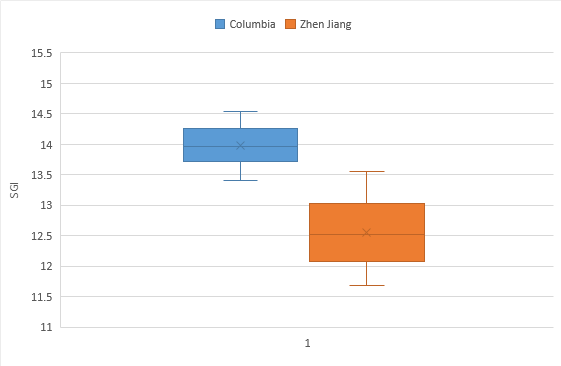
\includegraphics[height=8cm]{boxplot.png}}
\centerline{Figure2:boxplot}
As is shown in the figure of statistics, the SGI of Columbia.SC is generally higher than that of Zhenjiang. The SGI of Zhenjiang is more sensitive to that of Columbia.SC. The result proves that SGI of Zhenjiang benefits from some indictors in degrees. In other words, the development of Columbia.SC is more balanced than that of Zhenjiang.\\
\subsection{Selection of aggregation method}%subsection 6.2
In Task 1, we compare linear aggregation with geometric aggregation in advantages. For that reason, we finally decided to use linear aggregation to combine individual variables into the theme scores and geometric aggregation to combine theme scores into SGI.\\
We tried to use geometric aggregation to combine individual variables into the theme scores. And we observe that the calculated SGI using different data may varies in difference.\\
Our model is sensitive to the selection of aggregation method.\\

%Section 7
\section{Strengths and weaknesses}
\subsection{Strengths}%subsection 7.1
\begin{itemize}
\item Our model establishes a detailed group of 52 indictors, which reflects the ten principles for smart growth and the three E's of sustainability. On basis of this, we can assess the success of smart growth of a city.
\item In the construction of SGI model, we use linear aggregation to combine individual variables into the theme scores. Compensability of linear aggregation ensures fair assessment of different cities which have different emphasis in urban development. Then we use geometric aggregation to combine theme scores into SGI.Low compensability of geometric aggregation requires a city to develop evenly in all themes. 
\item We use entropy method to determine weights of indictors or themes, which avoid subjectivity.
\item SGI model has an all-round and objective assessment of the success of smart growth of a city.
\end{itemize}
\subsection{Weakness}%subsection 7.2
\begin{itemize}
\item In our model, we regard the relationship between initiative and indictor as one to one. In reality, a plan can result in the change in other indictors(not included in plan) because of correlation between indictors. The real SGI may be different with our calculated SGI.
\item In our model, we neglect the government's executive force.
\end{itemize}


\section{References}
\begin{thebibliography}{99}
\bibitem{1}Bannerjee,S.Bone,J.and Finger,Y.(2016).European Digital City Index-Methodology Report.Nesta Report-ISBN Number:978-1-84875-153-8
\bibitem{2}\url{http://www.wolframalpha.com/input/?i=columbia,+sc}
\bibitem{3}Jing Tan,Xiaoma Tao,Xu Chen.(2012).A Synthetic Measurement of Urban "Smart Growth" Based on Improved Entropy Method.Resources and Environment in the Yangtze Basin
\bibitem{4}Zhenjiang Statistical Yearbook,2014. Available at:\\
\url{http://tjj.zhenjiang.gov.cn/tjzl/tjnj/}
\bibitem{5}National Bureau of Statistics of China. Available at:\\
\url{http://data.stats.gov.cn/}
\bibitem{6}Data of Columbia.SC. Available at:\\
\url{http://www.city-data.com/city/Columbia-South-Carolina.html}
\bibitem{7}Yujuan Chen,Qifen Zha,Xiaolan Li.(2006).Application of Entropy Method in the Evaluation of Urban Sustainable Development.Journal of Jiangsu University(Social Science Edition)
\end{thebibliography}

\begin{appendices}
Here are  programmes we used in our model as follow.\\
\textbf{\textcolor[rgb]{0.98,0.00,0.00}{calculation of SGI matlab source:}}
\lstinputlisting[language=Matlab]{./code/model.m}
\textbf{\textcolor[rgb]{0.98,0.00,0.00}{calculation of weight by the entropy method matlab source:}}
\noindent{\lstinputlisting[language=Matlab]{./code/entropy.m}}
\end{appendices}

\end{document}